
\documentclass[compress]{beamer} %this is to use copressed header from the
\usepackage{etex}
\usepackage{beamerthemeshadow} %our theme, later you can change it
\usepackage[frenchb]{babel}
\usepackage{fancyhdr} % Required for custom headers
\usepackage[utf8]{inputenc}
\usepackage[lined,boxed]{algorithm2e}
\usepackage[all]{xy}
\usepackage{animate} %need the animate.sty file
\graphicspath{{./Figure/}} 
% editing header
\setbeamertemplate{headline}
{
  \leavevmode%
  \hbox{%
  \begin{beamercolorbox}[wd=.5\paperwidth,ht=2.25ex,dp=1.8ex,leftskip=1em,left]{section in head/foot}%
    \usebeamerfont{subsection in head/foot}\hspace*{5ex}\insertsectionhead
  \end{beamercolorbox}%
  \begin{beamercolorbox}[wd=.5\paperwidth,ht=2.25ex,dp=1.8ex,left,leftskip=1em]{subsection in head/foot}%
    \usebeamerfont{section in head/foot}\insertshorttitle\hspace*{2ex}
  \end{beamercolorbox}}%
  \vskip0pt%
}

% editing footer
\setbeamertemplate{footline}
{
  \leavevmode%
  \hbox{%
  \begin{beamercolorbox}[wd=.5\paperwidth,ht=2.25ex,dp=1ex,right]{author in head/foot}%
    \usebeamerfont{author in head/foot}\insertshortauthor\hspace*{2ex}
  \end{beamercolorbox}%
  \begin{beamercolorbox}[wd=.5\paperwidth,ht=2.25ex,dp=1ex,right]{date in head/foot}%
    \usebeamerfont{date in head/foot}\insertshortdate{}\hspace*{2em}
    \insertframenumber{} / \inserttotalframenumber\hspace*{2ex} 
  \end{beamercolorbox}}%
  \vskip0pt%
}
\definecolor{orange}{rgb}{1,0.5,0}
\definecolor{darkgreen}{rgb}{0,0.5,0}
\definecolor{darkblue}{rgb}{0,0,0.5}

\def\etal{et al.\ }
\def\ie{i.e.\ }
\def\eg{e.g.\ }

%put a wide hat over the argumetn
\newcommand{\lift}[1]{\ensuremath{\widehat{#1}}}

%put a wide hat over the argumetn
%\newcommand{\lifto}[1]{\ensuremath{\check{#1}}}
\newcommand{\lifto}[1]{\ensuremath{\overset{_{_{\circ}}}{#1}}}


% stack vector
\newcommand{\stackv}[1]{\ensuremath{\vet{v}\left( {#1} \right)}}
\newcommand{\ustackv}[1]{\ensuremath{\inv{\vet{v}}\left( {#1} \right)}}

% symmetric stack vector
\newcommand{\stackvs}[1]{\ensuremath{\vet{v}_{\textit{sym}}\left( {#1} \right)}}

% Matrix Lifting: put a wide hat over the argument intended to be a matrix
\newcommand{\mlift}[1]{\ensuremath{\lift{\mat{#1}}}}
\newcommand{\mlifto}[1]{\ensuremath{\lifto{\mat{#1}}}}

% Vector Lifting: put a wide hat over the argument intended to be a matrix
\newcommand{\vlift}[1]{\ensuremath{\lift{\vet{#1}}}}
\newcommand{\vlifto}[1]{\ensuremath{\lifto{\vet{#1}}}}

\newcommand{\bmat}[1]{\ensuremath{\begin{bmatrix} #1 \end{bmatrix}}}
% Vector: print the argument as a vector
\newcommand{\vet}[1]{\ensuremath{\mathbf{#1}}}

% Matrix: print the argument as a matrix
\newcommand{\mat}[1]{\ensuremath{\,\mathtt{#1}\,}}

% Inverse: print a -1 on the top right of the argument 
\newcommand{\inv}[1]{\ensuremath{{#1}^{\text{-}1}}}

% Inverse: print a -1 on the top right of the argument 
\newcommand{\minv}[1]{\ensuremath{\mat{{#1}}^{\text{-}1}}}

% Transpose: print a T on the top right of the argument 
\newcommand{\tra}[1]{\ensuremath{{#1}^{\!\mathsf{T}}}}

% Transpose Matrix: print a T on the top right of the argument intended to be a matrix 
\newcommand{\mtra}[1]{\ensuremath{\tra{\mat{#1}}}}

% Transpose Vector: print a T on the top right of the argument intended to be a vector
\newcommand{\vtra}[1]{\ensuremath{\tra{\vet{#1}}}}

% minus transpose:  print a -T on the top right of the argument
\newcommand{\ment}[1]{\ensuremath{{#1}^{\text{-}\mathsf{T}}}}

% minus transpose matrix:  print a -T on the top right of the argument
\newcommand{\mment}[1]{\ensuremath{{\mat{#1}}^{\text{-}\mathsf{T}}}}

% Cross Matrix:  print the argument in the cross matrix notation
\newcommand{\crmat}[1]{\ensuremath{\left[{#1}\right]_{\times}}}

%random variable
\newcommand{\rand}[1]{\ensuremath{\mathbb{#1}}}

%insert 2 figures on a row
\newcommand{\insertTwoF}[4]{
  \begin{figure}[h!]
    \centering
    \begin{minipage}{#4\linewidth}
    \includegraphics[width=\linewidth]{#1}
    \end{minipage}
    \begin{minipage}{#4\linewidth}
    \includegraphics[width=\linewidth]{#2}
    \end{minipage}
      \caption{#3}
  \end{figure}  
}

\newcommand{\insertF}[3]{
  \begin{figure}[h!]
    \centering
    \begin{minipage}{#3\linewidth}
    \includegraphics[width=\linewidth]{#1}
    \end{minipage}  
      \caption{#2}
  \end{figure}  
}

\newcommand{\bfE}{\mathbf{E}}
\newcommand{\bfz}{\mathbf{z}}

%enable numbering captions for the images
\setbeamertemplate{caption}[numbered]


%begining of the doc
\begin{document}

 \title{Building Detection Using Graph Cut}  
 %\author{Jia LI}
 %\date{August, 2013} 

 %title page
 \begin{frame}
\titlepage
    \centering
    \begin{minipage}{0.4\textwidth}
    \begin{flushleft} \large
    \emph{Author:}\\
    LI Jia\\
    XU Minmin\\
    
    \end{flushleft}
    \end{minipage}
    \begin{minipage}{0.4\textwidth}
    \begin{flushright} \large
    \emph{Course:}\\
    Méthodes avancées de traitement d'images 
    \end{flushright}
    \end{minipage}\\[3cm]
 \end{frame}

 \section{Plan}
 \begin{frame}
  \scriptsize
  {
  \begin{enumerate}
  \item Grab cut 
    \begin{enumerate}
     \item approach
     \item synthetic test
    \end{enumerate}
  \item Automation
    \begin{enumerate}
     \item shadow detection
     \item vegetation detection
     \item ROI region
     \item Foreground region
    \end{enumerate}
  \end{enumerate}
  %\frametitle{Table of contents}
  %\tableofcontents
  }
 \end{frame} 
 
 \section{Introduction}
 \begin{frame}
  \frametitle{Motivation}
  \begin{itemize}
   \item Application : urban monitoring, change detection, estimation of human population, etc.
   \item Challenging : complex background, without human interacting.
  \end{itemize}
  \insertF{vatican-city-satellite-image-ikonos-high-resolution}{Example of Arian Urban Image}{0.4}
 \end{frame}

 \begin{frame}
  \frametitle{Intuition}
  Approach proposed by Ok {\textit{et. al}} \cite{Ok:2013} : 
  \begin{itemize}
   \item Grab cut (Rother \cite{Rother:2004}) : semi-automatic segmentation, with a user defined foreground-background window.
   \insertTwoF{grab_cut}{grab_cut_result}{Grab cut method illustration}{0.45}
   \item Foreground-background estimation : prior knowledge, shadow, vegetation ...
  \end{itemize}
 \end{frame}

 \section{Grab Cut}
 \begin{frame}
  \scriptsize
  {
  \begin{enumerate}
  \item \textbf{Grab Cut} 
    \begin{enumerate}
     \item Approach
     \item Experience
    \end{enumerate}
  \item Automation
    \begin{enumerate}
     \item shadow detection
     \item vegetation detection
     \item ROI region
     \item Foreground region
    \end{enumerate}
  \end{enumerate}
  %\frametitle{Table of contents}
  %\tableofcontents
  }
 \end{frame}  
 
 \section{Approach}
 \begin{frame}
  \frametitle{Image Segmentation by Graph Cut}
  Gibb's energy for image segmentation :
  \[
  \bfE(\alpha,\theta,\bfz)=U(\alpha,\theta,\bfz)+V(\alpha,\bfz)
  \]
  \begin{itemize}
   \item<1> $\bfz=(z_1,z_2,...,z_N)$, a $N$-pixel image.
   \item<1> $\alpha=(\alpha_1,\alpha_2,...,\alpha_N)$ label for each pixel, typically $\alpha_n\in\{0,1\}$.
   \item<1> $\theta$, background model for each label/class, empirical histogram, GMM...
  \end{itemize}
 \end{frame}

 \begin{frame}
  \frametitle{Image Segmentation by Graph Cut}
  Gibb's energy for image segmentation :
  \[
  \bfE(\alpha,\theta,\bfz)=U(\alpha,\theta,\bfz)+V(\alpha,\bfz)
  \]
  \begin{itemize}
  \item $U=\sum_n -\log(p_\theta (\alpha_n,z_n))$ the likelihood term.
  \item $V=\gamma \sum_{n,m\in \mathbf{C}}[\alpha_m \neq \alpha_n] \exp(-\beta|z_n-z_m|^2)$ the regularity term, $\beta=0$ correspond to the Isings model.
  \end{itemize}

  Segmentation : $\hat \alpha= \arg\min\limits_\alpha \bfE(\alpha,\theta)$ 
  \begin{itemize}
   \item Standard graph cut for minimization. ([Boykov and Jolly 2001; Kolmogorov and Zabih 2002]) 
  \end{itemize}
 \end{frame}
 
 \begin{frame}
  \frametitle{Grab Cut}
  Grab cut for foreground background separation:
  \begin{itemize}
   \item GMM for the likelihood term. One GMM for the foreground and the other for the background.
   \item Iterative estimation and parameters learning instead of a one-shot minimization.
   \item Relaxed user interactive labeling.
  \end{itemize}
  \insertTwoF{graph_label}{grab_label}{Illustration of Graph cut and Grab cut labeling. (Rother 2004 \cite{Rother:2004})}{0.4}
 \end{frame}

 
 \begin{frame}
  \frametitle{Grab Cut}
  Energy for grab cut : 
  \[
  \bfE(\alpha,\mathbf{k},\theta,\bfz)=U(\alpha,\mathbf{k},\theta,\bfz)+V(\alpha,\bfz)
  \]

 \begin{itemize}
  \item $\mathbf{k}=(k_1,k_2,...,k_N)$, with $k_n\in \{1,...,K\}$ assigning each pixel to a GMM component.
  \item $U(\alpha,\mathbf{k},\theta,\bfz)=\sum_n D_n(\alpha,\mathbf{k},\theta,\bfz)$, with 
  \[
  \begin{split}
  D_n(\alpha,\mathbf{k},\theta,\bfz)&=-\log(p_\theta (\alpha_n,k_n,z_n)) -\log(\pi(\alpha_n,k_n)) \\
  &=-\log(\pi(\alpha_n,k_n))-1/2\log \det \Sigma(\alpha_n,k_n)\\
  &-1/2 \tra{[z_n-\mu(\alpha_n,k_n)]}\inv{\Sigma(\alpha_n,k_n)}[z_n-\mu(\alpha_n,k_n)]
  \end{split}
  \]

 \end{itemize}
 \end{frame}
 
 \begin{frame}
  \frametitle{Minimization Algorithm}
  \begin{enumerate}
   \item \textit{Initialization}. $\alpha_n=1$ for $n\in \mathbf{T}_u$, $\alpha_n=0$ otherwise.
   \item \textit{Learning}. $\mathbf{k}=\arg\min\limits_{\mathbf{k}} U(\alpha,\mathbf{k},\theta,\bfz)$, $\theta=\arg\min\limits_{\theta} U(\alpha,\mathbf{k},\theta,\bfz)$
   \item \textit{Estimation}. $\min\limits_{\alpha}\min\limits_{\mathbf{k}}\bfE(\alpha,\mathbf{k},\theta,\bfz) $
   \item \textit{Iteration}. Repeat 2,3 until convergence.
  \end{enumerate}
  \begin{figure}[h!]
    \centering
    \begin{minipage}{0.27\linewidth}
    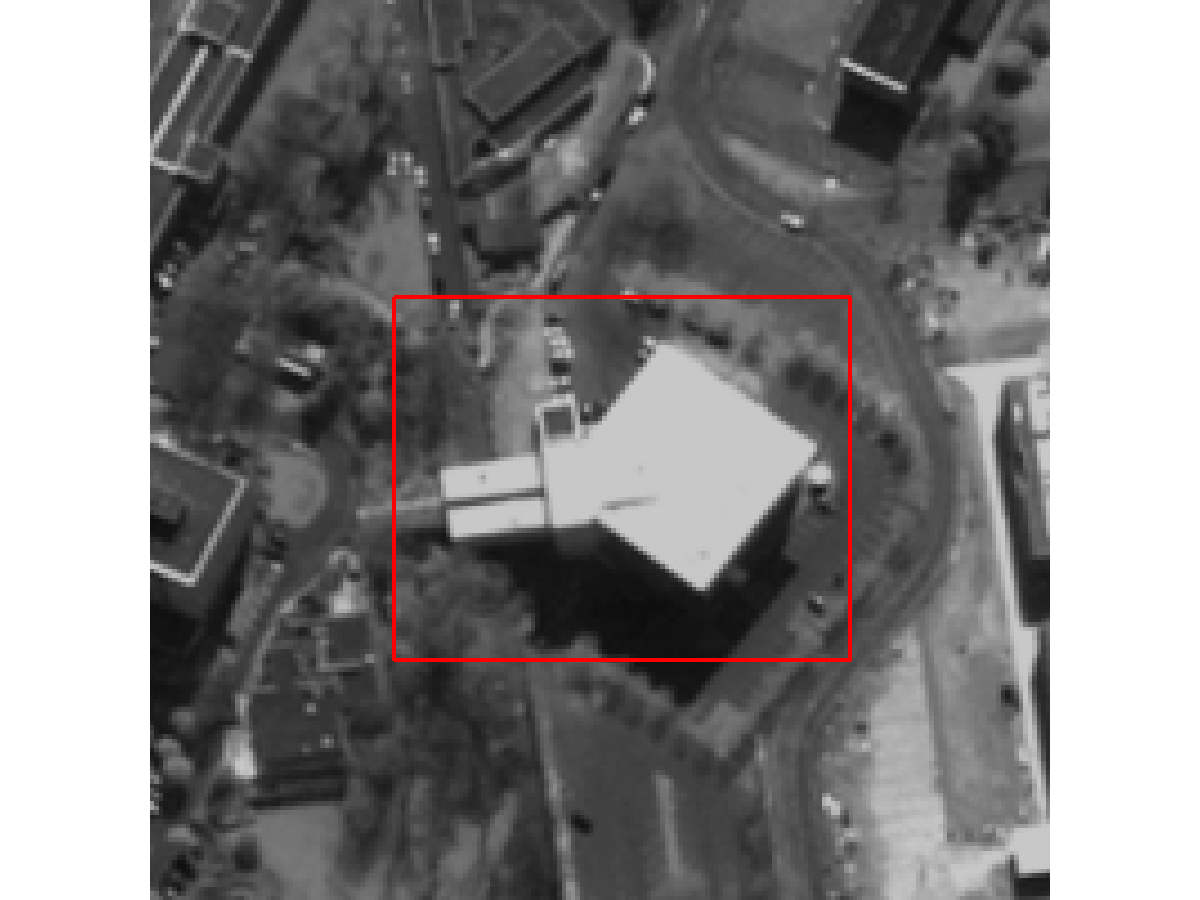
\includegraphics[width=\linewidth]{init}
    \end{minipage}
    \begin{minipage}{0.27\linewidth}
    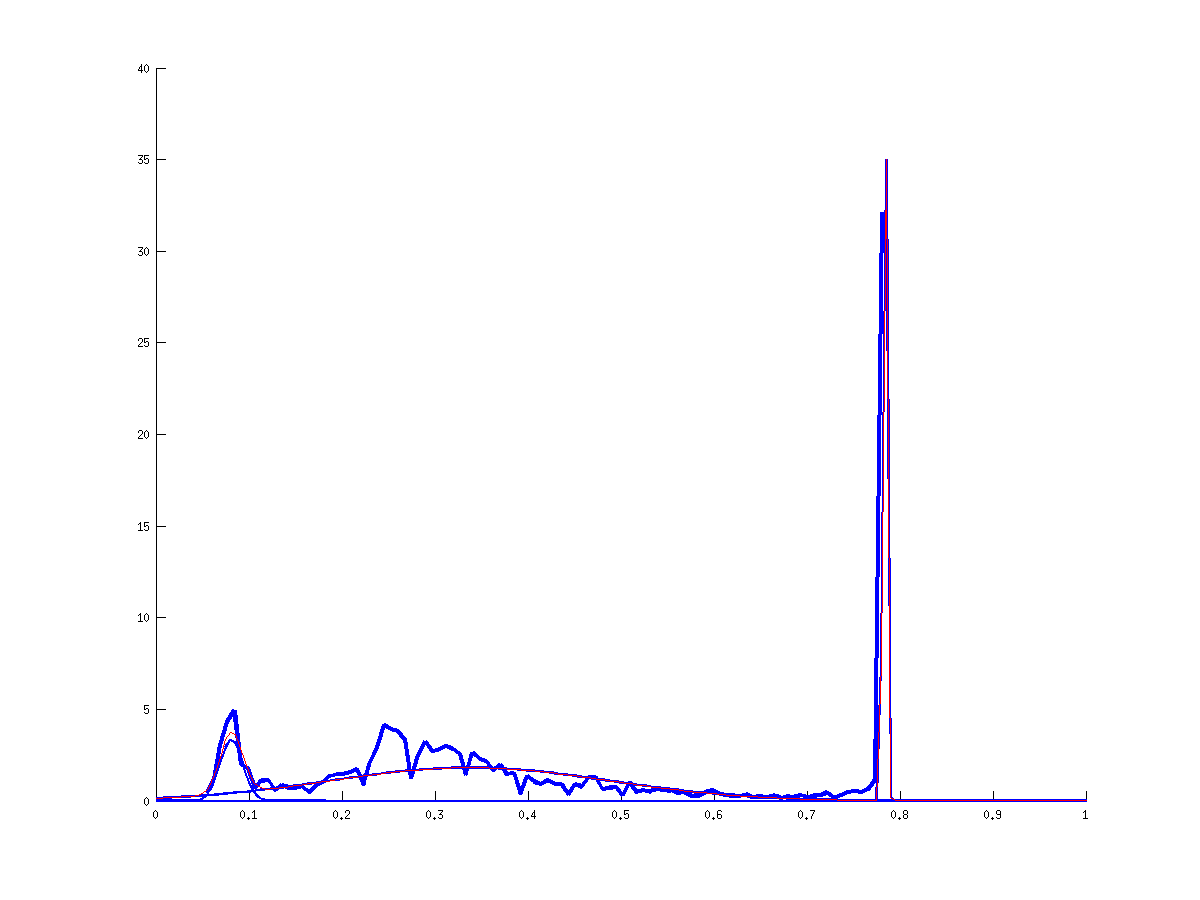
\includegraphics[width=\linewidth]{fore_hist}
    \end{minipage}
    \begin{minipage}{0.27\linewidth}
    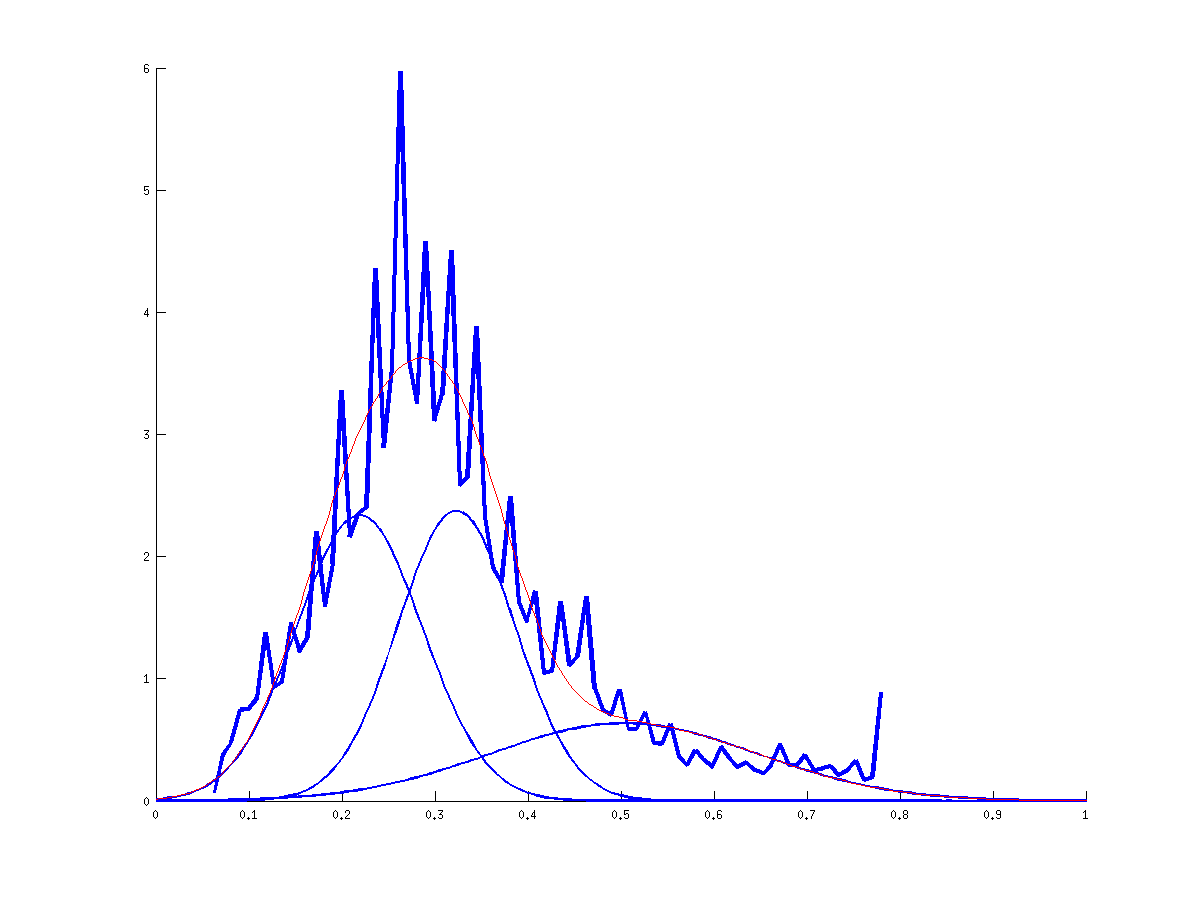
\includegraphics[width=\linewidth]{back_hist}
    \end{minipage}
    \begin{minipage}{0.27\linewidth}
    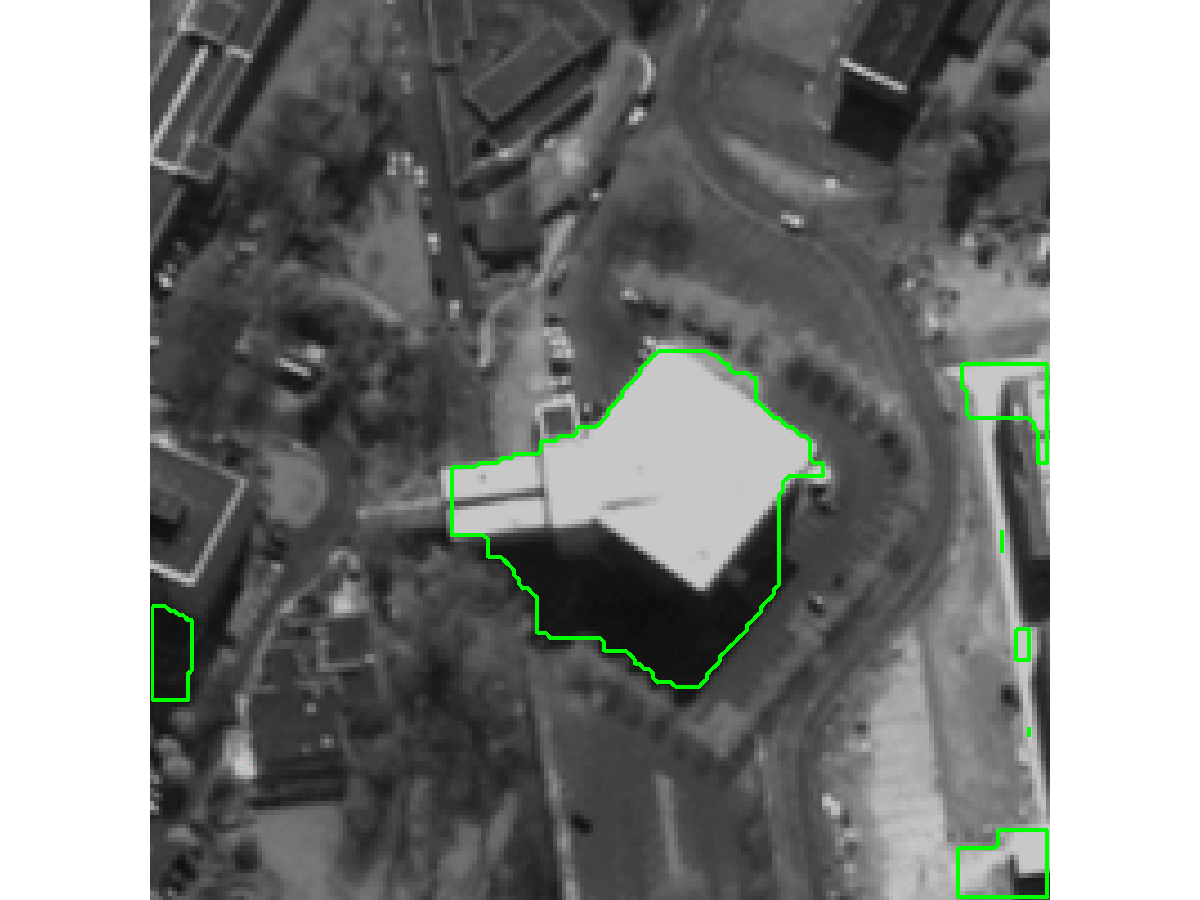
\includegraphics[width=\linewidth]{result_1}
    \end{minipage}
    \begin{minipage}{0.27\linewidth}
    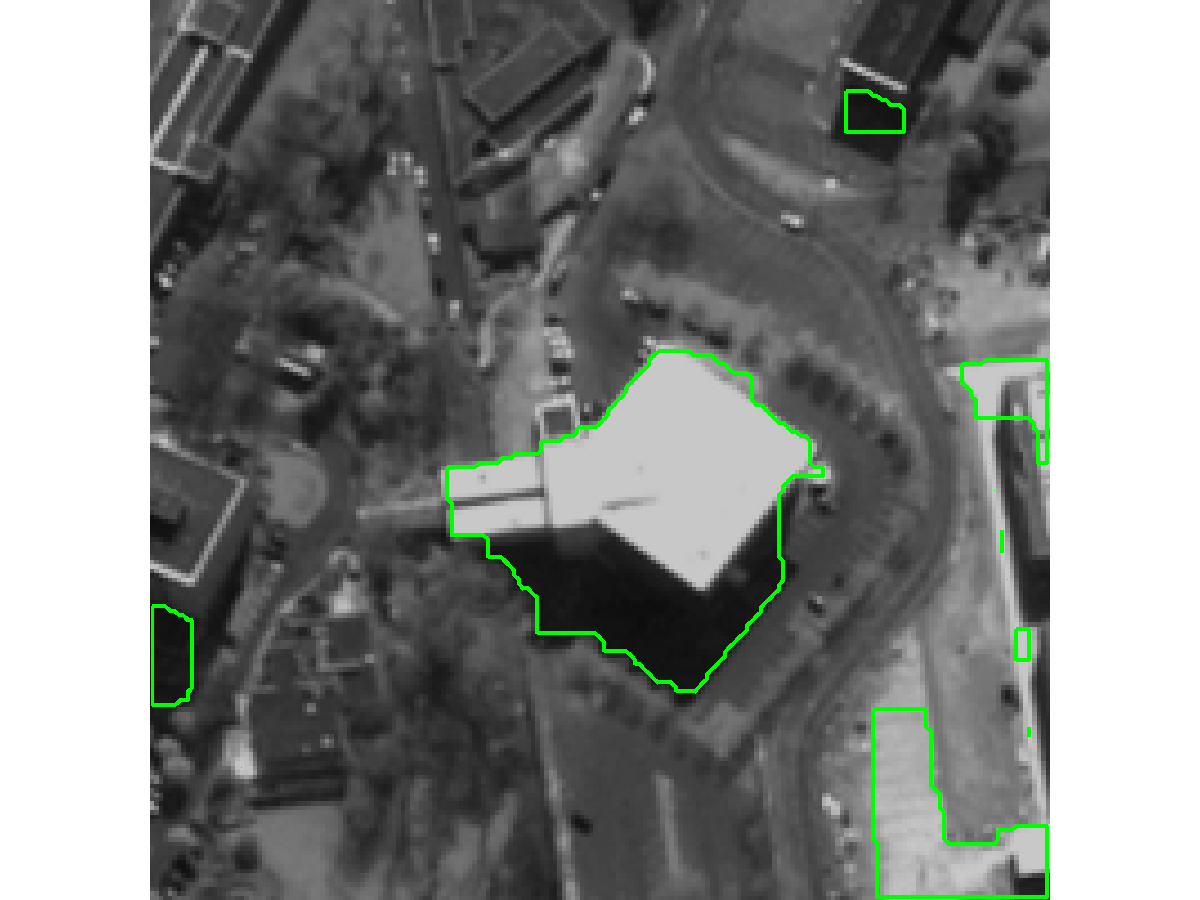
\includegraphics[width=\linewidth]{result_2}
    \end{minipage}    
    \begin{minipage}{0.27\linewidth}
    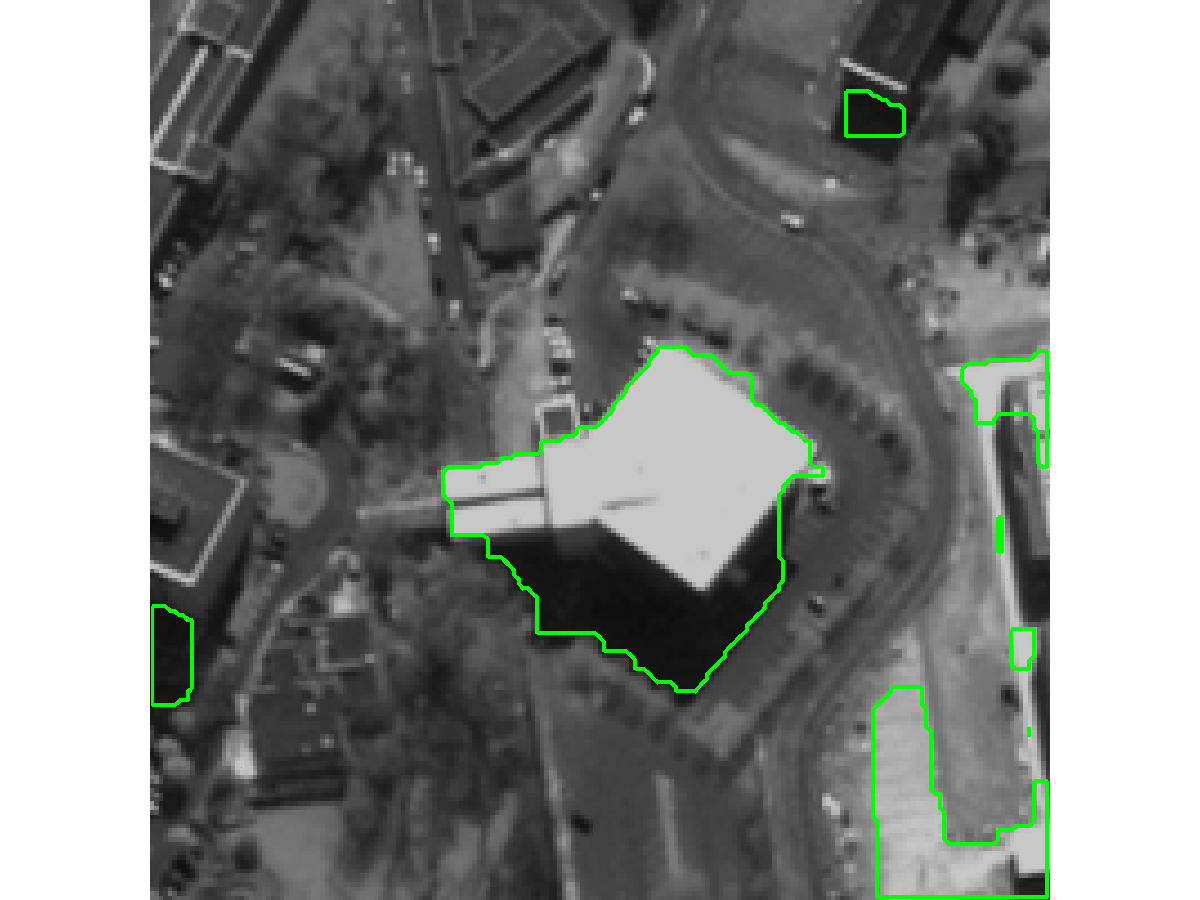
\includegraphics[width=\linewidth]{result_3}
    \end{minipage} 
      \caption{Illustration of the algorithm}
  \end{figure}  
 \end{frame}
 
 

\section{Automation}
 \begin{frame}
  \scriptsize
  {
  \begin{enumerate}
  \item {Grab Cut} 
    \begin{enumerate}
     \item Approach
     \item Experience
    \end{enumerate}
  \item \textbf{Automation}
    \begin{enumerate}
     \item shadow detection
     \item vegetation detection
     \item Foreground region
     \item ROI region
    \end{enumerate}
  \end{enumerate}
  %\frametitle{Table of contents}
  %\tableofcontents
  }
 \end{frame}   
 
\section{shadow detection}
\begin{frame}
  \frametitle{shadow detection}
   Two steps: K-means and growth of region 
  \begin{itemize}
   \item Use K-means to find the first peak and therefore find a simple threshold for shadows.
  
   \item Use the result of threshold as seed to apply method of growth of region to obtain the complete shadows.
    \insertF{shadow}{Shadow detection}{0.5}
  \end{itemize}
 \end{frame} 
 
 \section{vegetation detection}
\begin{frame}
  \frametitle{vegetation detection}
  \begin{itemize}
   \item Likelihood between the color and the color of vegetation.
   \end{itemize}
   \insertF{vegetation}{Vegetation detection}{0.8}
 \end{frame} 
 
  \section{Clean shadows}
\begin{frame}
  \frametitle{Clean shadows}
  \begin{itemize}
   \item First remove the detected vegetation from the shadow.
   \item Remove the shadow corresponding to the detected vegetation by double threshold of fuzzy map on each connected component.
   \insertF{cleaned_shadow}{Cleaned shadow}{0.5}
  \end{itemize}
 \end{frame} 
 
 \section{Foreground detection}
\begin{frame}
  \frametitle{Foreground detection}
    
  \begin{itemize}
   \item Construct shadow structural element with reversed sun direction and length of shadow.
   
   \item Create the fuzzy map and then apply the double threshold to obtain the foreground mask.
   \insertTwoF{fuzzy_map}{fore-back}{Fuzzy map and Foreground detection}{0.4}
  \end{itemize}
 \end{frame} 
 
 
 \section{ROI detection}
\begin{frame}
  \frametitle{ROI detection}
    
  \begin{itemize}
   \item Construct shadow structural element with reversed sun direction and length to be configured.
   \insertF{re_direction}{Structural element}{0.5}
   \end{itemize}
 \end{frame} 
 
   \section{ROI detection}
\begin{frame}
\begin{itemize}
  \frametitle{ROI detection}
   \item Dilate the shadow with the shadow structural element in order to obtain the regions of interest(in which there are buildings we want to detect).
   \insertF{ROI}{Region of interest}{0.8}
  \end{itemize}
 \end{frame} 
 
 \section{Experience}
  \begin{frame}
   {\Huge
     \vspace {0.15\textwidth}
     \begin{columns}
       \begin{column}{0.3\textwidth}
       \end{column}
       \begin{column}{0.3\textwidth}
        \text{Thank you!}
       \end{column}
       \begin{column}{0.3\textwidth}
       \end{column}
     \end{columns}
   }
   \vspace {0.025\textwidth}
   \begin{center}
   {\huge Q\&A}
   \end{center}
 \end{frame}

\begin{frame}\frametitle{References}
\frametitle{References}
\bibliographystyle{splncs}
\bibliography{graph}
\end{frame}

\end{document}